\documentclass[16pt]{beamer}

\ifdefined\chinchin
\usepackage[CJKspace]{xeCJK}
\setCJKmainfont[BoldFont=SimHei,ItalicFont=AR PL KaitiM GB]{SimSun}
\newcommand{\cc}[2]{#1}
\else
\newcommand{\cc}[2]{#2}
\fi

%\usepackage{newtxtext,newtxmath}	% use Times Roman font
%\usepackage{newtxtext}
%\renewcommand{\familydefault}{\sfdefault}
%\usefonttheme{serif}
\usefonttheme{professionalfonts}
%\setbeamertemplate{theorems}[numbered]
\setbeamertemplate{caption}{\insertcaption} 	% no `Figure' prefix before caption

\mode<presentation> {

%\usetheme{default}
%\usetheme{AnnArbor}
%\usetheme{Antibes}
%\usetheme{Bergen}
%\usetheme{Berkeley}
%\usetheme{Berlin}
%\usetheme{Boadilla}
%\usetheme{CambridgeUS}
%\usetheme{Copenhagen}
%\usetheme{Darmstadt}
%\usetheme{Dresden}
%\usetheme{Frankfurt}
%\usetheme{Goettingen}
%\usetheme{Hannover}
%\usetheme{Ilmenau}
%\usetheme{JuanLesPins}
%\usetheme{Luebeck}
\usetheme{Madrid}
%\usetheme{Malmoe}
%\usetheme{Marburg}
%\usetheme{Montpellier}
%\usetheme{PaloAlto}
%\usetheme{Pittsburgh}
%\usetheme{Rochester}
%\usetheme{Singapore}
%\usetheme{Szeged}
%\usetheme{Warsaw}

%\usecolortheme{albatross}
%\usecolortheme{beaver}
%\usecolortheme{beetle}
%\usecolortheme{crane}
%\usecolortheme{dolphin}
%\usecolortheme{dove}
%\usecolortheme{fly}
%\usecolortheme{lily}
\usecolortheme{orchid}
%\usecolortheme{rose}
%\usecolortheme{seagull}
%\usecolortheme{seahorse}
%\usecolortheme{whale}
%\usecolortheme{wolverine}		% Hofstra

%\setbeamertemplate{footline} % To remove the footer line in all slides uncomment this line
\setbeamertemplate{footline}[page number] % To replace the footer line in all slides with a simple slide count uncomment this line
\setbeamertemplate{navigation symbols}{} % To remove the navigation symbols from the bottom of all slides uncomment this line
}

\setbeamertemplate{headline}{}
\setbeamersize{text margin left=1mm,text margin right=1mm} 
\settowidth{\leftmargini}{\usebeamertemplate{itemize item}}
\addtolength{\leftmargini}{\labelsep}

\usepackage[backend=biber,style=numeric]{biblatex}
\bibliography{../AGI-book}
\renewcommand*{\bibfont}{\footnotesize}
\setbeamertemplate{bibliography item}[text]

\usepackage{graphicx} % Allows including images
\usepackage{tikz-cd}
\usepackage[export]{adjustbox}% http://ctan.org/pkg/adjustbox
\usepackage{verbatim} % comments
% \usepackage{tikz-cd}  % commutative diagrams
% \newcommand{\tikzmark}[1]{\tikz[overlay,remember picture] \node (#1) {};}
% \usepackage{booktabs} % Allows the use of \toprule, \midrule and \bottomrule in tables
% \usepackage{amssymb}  % \leftrightharpoons
\usepackage{wasysym} % frownie face
\usepackage{newtxtext,newtxmath}	% Times New Roman font

\newcommand{\emp}[1]{{\color{violet}#1}}
\newcommand{\vect}[1]{\boldsymbol{#1}}
\newcommand{\tab}{\hspace*{1cm}}
\newcommand*\confoundFace{$\vcenter{\hbox{\includegraphics[scale=0.2]{../confounded-face.jpg}}}$}
\renewcommand{\smiley}{$\vcenter{\hbox{\includegraphics[scale=0.05]{../smiling-face.png}}}$}

%%%%%%%% Make table of contents %%%%%%%

\makeatletter
\renewcommand{\boxed}[1]{\fbox{\m@th$\displaystyle\scalebox{0.9}{#1}$} \,}
\makeatother
\newif\ifframeinlbf
\frameinlbftrue
\makeatletter
\newcommand\listofframes{\@starttoc{lbf}}
\makeatother
\addtobeamertemplate{frametitle}{}{%
	\ifframeinlbf
	\addcontentsline{lbf}{section}{\protect\makebox[2em][l]{%
			\protect\usebeamercolor[fg]{structure}\insertframenumber\hfill}%
		\insertframetitle\par}%
	\else\fi
}

%----------------------------------------------------------------------------------------
%	TITLE PAGE
%----------------------------------------------------------------------------------------

\title[The road to AGI]{\Huge《The road to AGI》}
\author{\cc{YKY 甄景贤}{YKY}} % Your name
%\institute[] % Your institution as it will appear on the bottom of every slide, may be shorthand to save space
%{
%Independent researcher, Hong Kong \\ % Your institution for the title page
%\medskip
%\textit{generic.intelligence@gmail.com} % Your email address
%}
\date{\today} % Date, can be changed to a custom date

\begin{document}

\frameinlbffalse
\addtocounter{page}{-1}
\begin{frame}[plain,noframenumbering]
\titlepage
\end{frame}

\addtocounter{page}{-1}
\begin{frame}[noframenumbering]
\frametitle{Table of contents}
\listofframes
\vspace*{0.5cm}
多谢 支持 \smiley
\end{frame}

%----------------------------------------------------------------------------------------
%	PRESENTATION SLIDES
%----------------------------------------------------------------------------------------

%------------------------------------------------

\frameinlbftrue
\begin{frame}
\frametitle{BERT 的革命性意义}
\begin{itemize}
	\item BERT 利用平常的文本 induce 出知识,而这 representation 具有 \emp{通用性 (universality)} :
	\begin{equation}
	\vcenter{\hbox{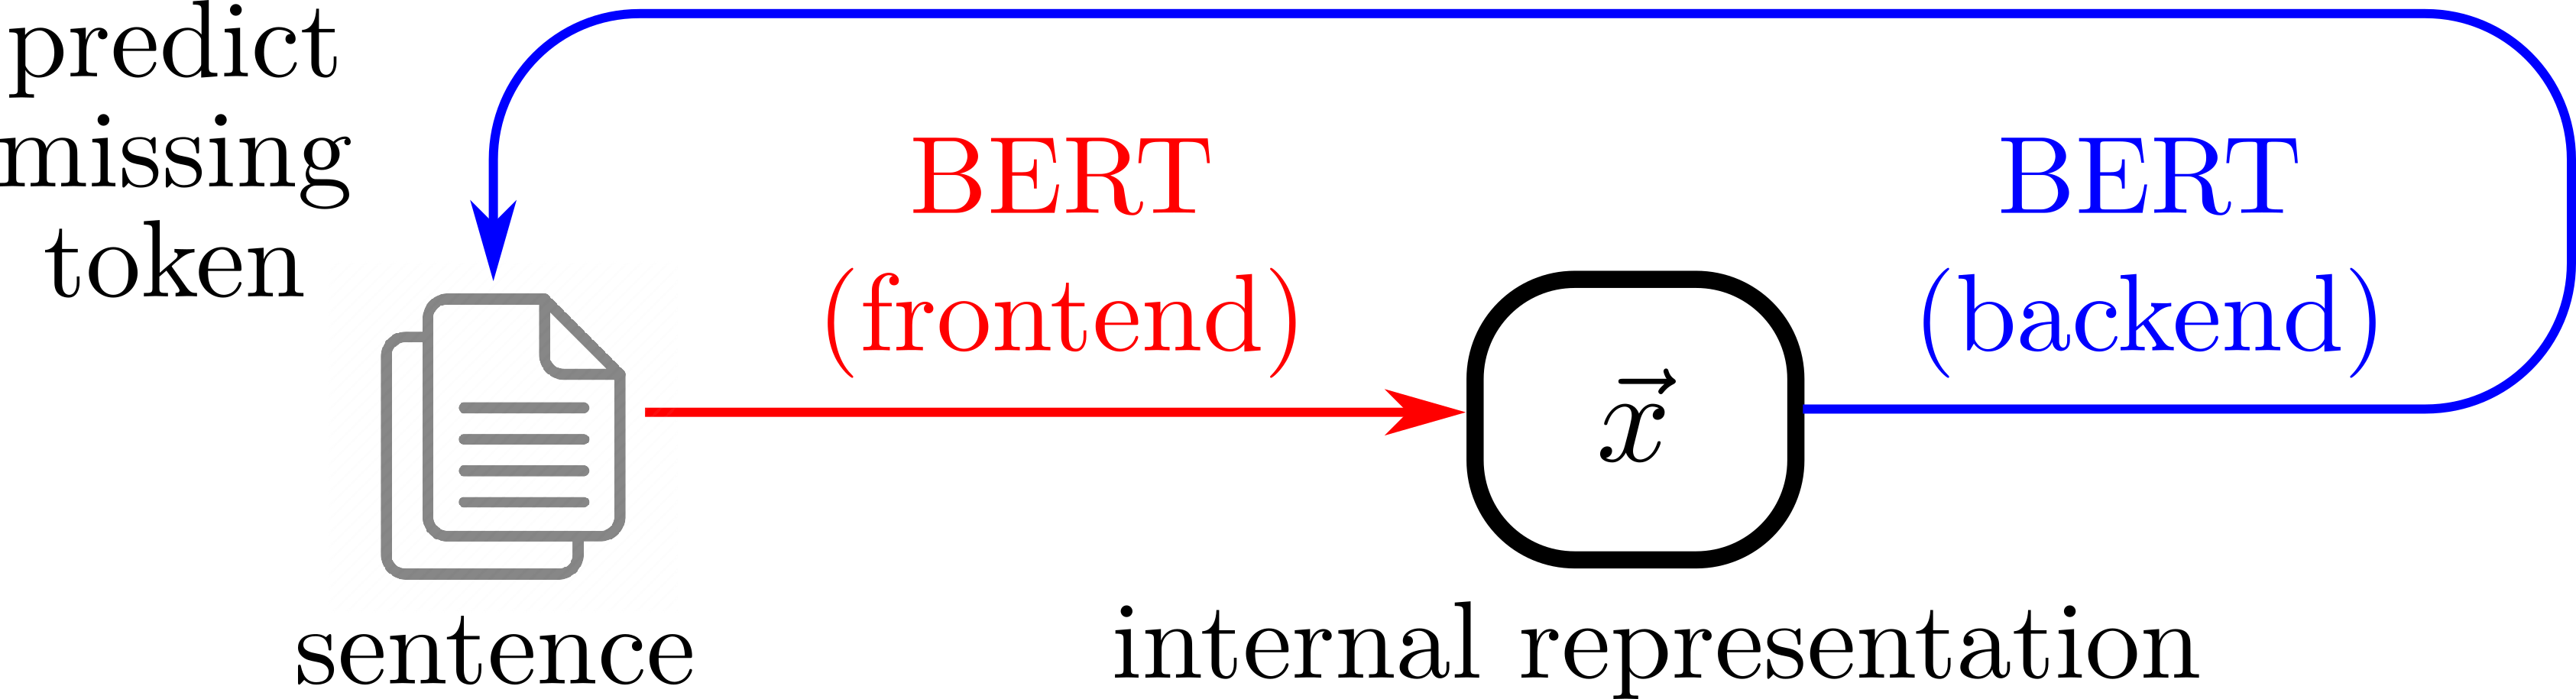
\includegraphics[scale=0.5]{BERT-architecture.png}}}
	\end{equation}
	换句话说: 隐状态的 representation 压缩了句子的意思,而它可以应用在别的场景下
	
	\item This implies that human-level AI can be \textit{induced} from existing corpora, 而\emp{不需要重复像人类婴儿成长的学习阶段}
	
	\item Such corpora can include items such as images, movies with dialogues / subtitles
	
	\item 这种训练方法是较早的另一篇论文提出,它并不属於 BERT 的内部结构
\end{itemize}
\end{frame}

\begin{frame}
\frametitle{从 BERT 过渡到 AGI}
\begin{itemize}
	\item \emp{词语} 组成 \emp{句子},类比於 逻辑中,\emp{概念} 组成 \emp{逻辑命题}
	
	\item 抽象地说,逻辑语言 可以看成是一种有 2个运算的 \emp{代数结构},可以看成是 加法 $\wedge$ 和 乘法 $\cdot$,其中 乘法 是不可交换的,但加法 可交换

	\item 例如 两个命题:
	\begin{equation}
	\mbox{我} \cdot \mbox{爱} \cdot \mbox{妳} \; \wedge \; \mbox{妳} \cdot \mbox{爱} \cdot \mbox{我}
	\end{equation}

	\definecolor{darkgreen}{rgb}{0.1, 0.5, 0.2}
	\item 这种逻辑结构 可以用 \emp{两层} 的 BERT 模型 处理:
	\begin{equation}
	\vcenter{\hbox{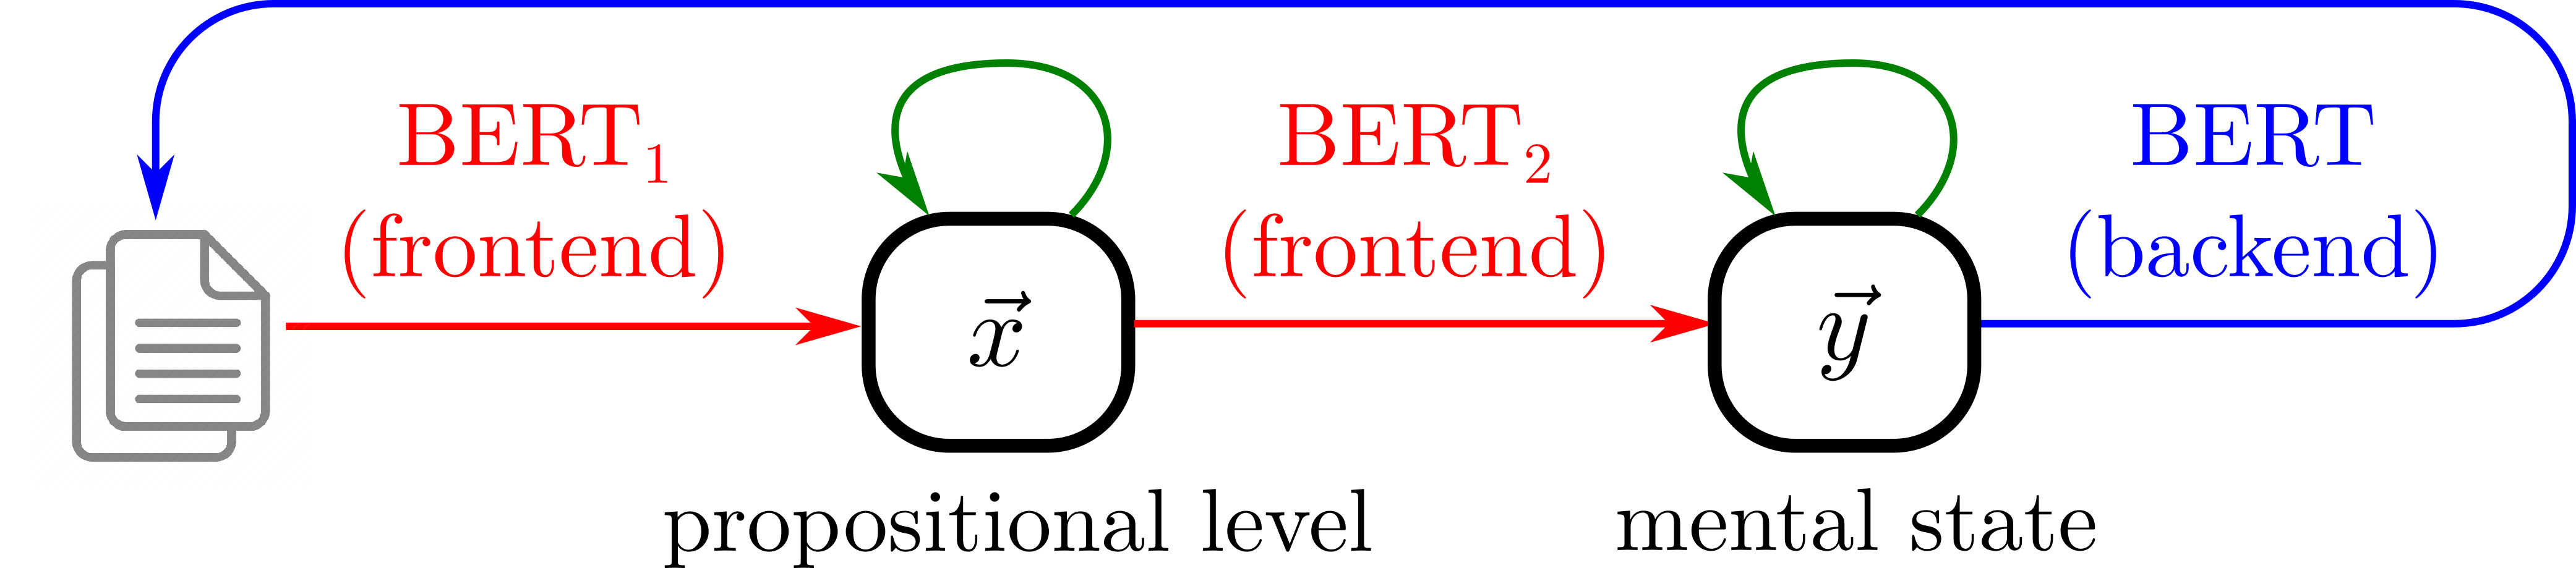
\includegraphics[scale=0.5]{2-BERT-architecture.png}}}
	\end{equation}
	({\color{red}第一层}似乎可以纳入到{\color{darkgreen}第二层},简化整个模型)

	\item 我发现 最难处理的问题,是在第2层 的状态 $\vec{x}$.  它是一个 逻辑命题 的 \emp{集合},集合中元素有可交换性,亦即 \emp{permutation invariance}.  这看似简单的特性,其实带来很大的麻烦

	% \item 如何 standardize 输入空间,使之可以接受任何形式的输入?
	
	% \item BERT 后端的输出可以是 actions,变成一个可以行动的 agent.  如何找大量的资料 训练它?

	% \item state $\vec{x}$ 的结构: 用 vector 还是 graph $\cong$ set of logic propositions 比较好? \\
	% 后者有 内在的 逻辑结构,是一种 inductive bias

	% \item 现时,所有 知识存在於 BERT 的 weights 里面,可不可以将一部分记忆 转化成 declarative knowledge,储存在 knowledge graph? 这做法有没有好处? 
\end{itemize}
\end{frame}

\begin{frame}
\frametitle{「集」结构 带来麻烦}
\begin{itemize}
	\item Word2Vec 也是革命性的; 由 Word2Vec 演变成 Sentence2Vec 则比较容易,基本上只是 向量的 \emp{延长} (concatenation); 逻辑命题 类似於 sentence

	\item 假设 全体逻辑命题的空间是 $\mathbb{P}$,则 \emp{命题集合} 的空间是 $2^{\mathbb{P}}$,非常庞大
	
	\item 如果限制 状态 $\vec{x}$ = working memory 只有 10 个命题,$\vec{x}$ 的空间是 $\mathbb{P}^{10}/\sim$ 其中 $\sim$ 是对称群 $\mathfrak{S}_{10}$ 的等价关系。 换句话说 $ 2^{\mathbb{P}} \cong \coprod_{n=0}^{\infty} \; \mathbb{P}^n / \mathfrak{S}_n $
	
	\item $\mathbb{P}^n / \mathfrak{S}_n$ 虽然是 $\mathbb{P}^n$ 的商空间,但 $\mathfrak{S}_n$-不变性 很难用神经网络实现

	\definecolor{darkgreen}{rgb}{0.1, 0.7, 0.2}
	\item 现时 比较可行的办法,是将 状态 $\vec{x}$ 实现成 一个时间上的「轮盘」,每个 ${\color{darkgreen}\bullet}$ 表示一个命题:
	\begin{equation}
	\vcenter{\hbox{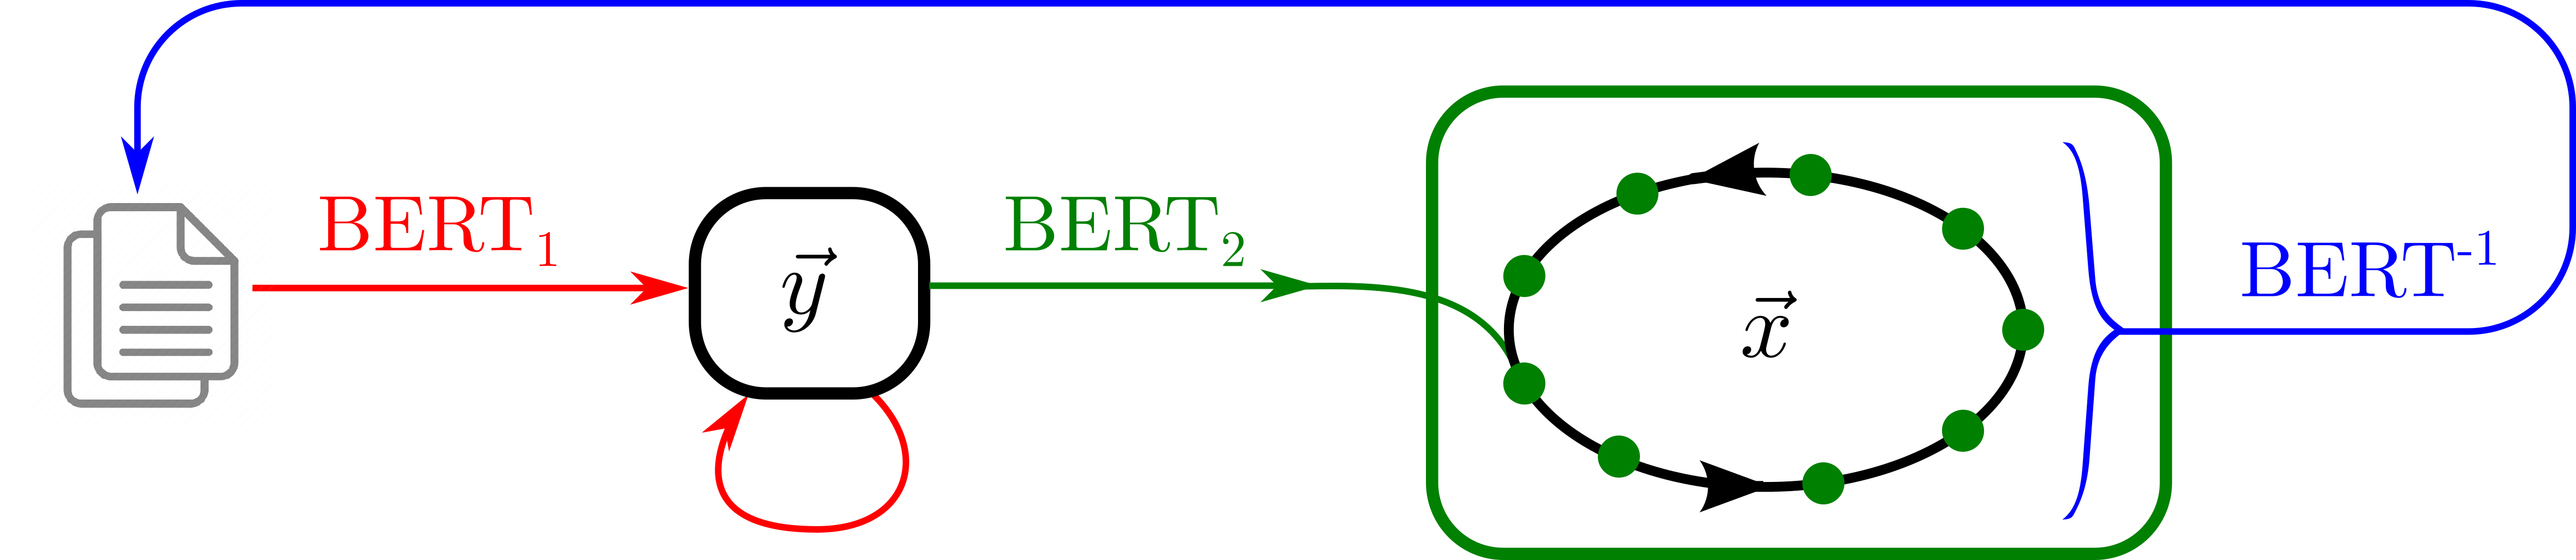
\includegraphics[scale=0.5]{BERT-with-carousel-architecture-1.png}}}
	\end{equation}

	\item 有趣的是,如果用「轮盘」方法,BERT 的 \emp{注意力机制} 有特殊意义....
\end{itemize}
\end{frame}

\begin{frame}
\frametitle{Attention 是什么?}
\begin{itemize}
	\item 注意力 最初起源於 Seq2seq,后来 BERT 引入 self-attention

	\item 在 Seq2seq 中,编码器 (encoder) 由下式给出,它将输入的词语 $x_i$ 转化成 一连串的 隐状态 $h_i$:
	\begin{equation}
	h_t = \mbox{RNN}_{encode}(x_t, h_{t-1})
	\end{equation}

	\item 这些 $h_i$ 可以综合成单一个 隐状态 $c = q(h_1, ..., h_n)$. 

	\item 这个 $c$ 被「寄予厚望」,它浓缩了整个句子的意义
	
	\item 解码器 的结构类似,它的隐状态是 $s_t$,输出 $y_t$:
	\begin{equation}
	s_t = \mbox{RNN}_{decode}(y_t, s_{t-1}, c_t)
	\end{equation}
	
	\item 注意最后的 $c_t$ 依赖时间,它是隐状态 $h_j$ 的 \emp{加权平均}:
	\begin{equation}
	c_i = \sum_j \alpha_{ij} h_j
	\end{equation}
	
	\item 其中 $\alpha_{ij}$ 量度 输入/输出 的隐状态之间的 \emp{相似度},取其最大值:
	\begin{equation}
	\alpha_{ij} = \mbox{softmax} \{ \langle s_i, h_j \rangle \}
	\end{equation}
	换句话说,$\alpha_{ij}$ \emp{选择} 最接近 $h_j$ 的 $s_i$
\end{itemize}
\end{frame}

\begin{frame}
\frametitle{Attention 在逻辑中的用处}
我这样理解 attention:
\begin{itemize}
	\item 例如,翻译时,输入/输出句子中「动词」的位置可以是不同的
	
	\item 当 解码器需要一个「动词」时,它的隐状态 $s_t$ 含有「动词」的意思
	
	\item Attention 机制 找出最接近「动词」的 编码器的隐状态 (可以 $\ge 1$ 个)$\sum h_j$,交给 解码器,这是一种 \emp{information retrieval}
	
	\item 例如,将 $M$ 件东西 映射 到 $N$ 件东西,可以有 $N^M$ 个 mappings,这是非常庞大的空间。 但如果这些物件有 \emp{类别},而\underline{同类只映射到同类},则可以用 attention 简化 mappings
	
	\item 所以 attention 是一种 inductive bias,它大大地缩小 mapping 空间

	\item 在逻辑的场景下,需要的 mapping 是 $f: \mbox{命题集合} \rightarrow \mbox{命题}$
	\begin{equation}
	\vcenter{\hbox{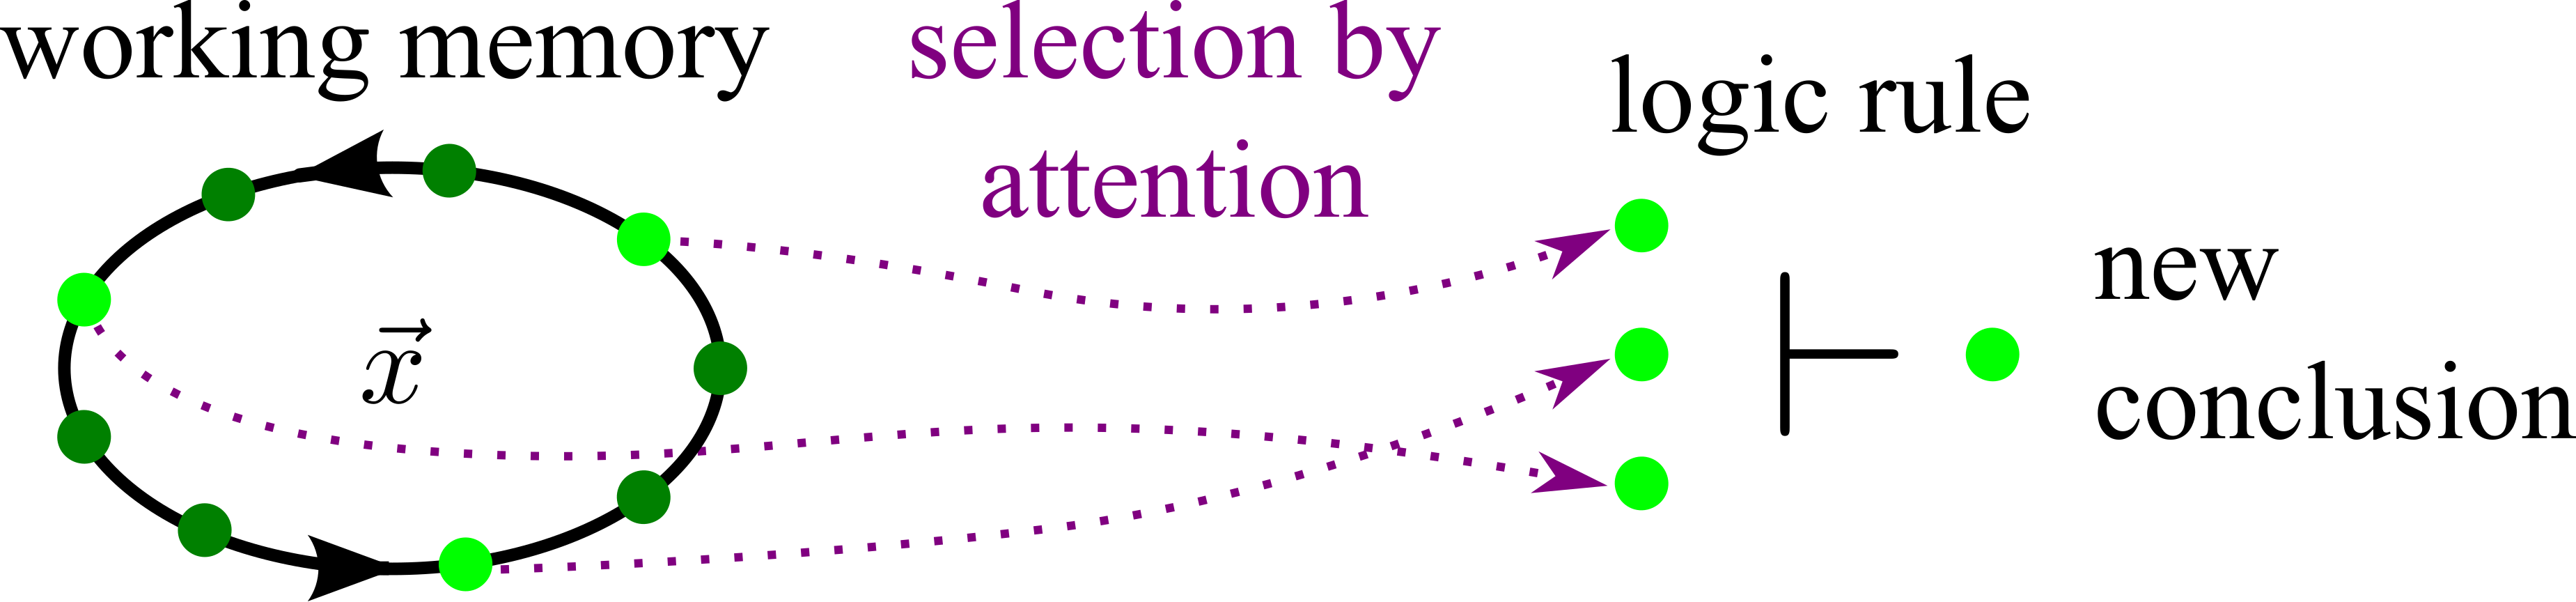
\includegraphics[scale=0.5]{attention-in-logic.png}}}
	\end{equation}

\end{itemize}
\end{frame}

\begin{frame}[plain]
\frametitle{要设计一种新的 attention}
\begin{itemize}
	\item 逻辑 attention 和 传统 attention 要求略有不同,这是关键的一步

	\item 不是「同类映射到同类」,而是要在庞大的 logic rules 空间中找到适用(applicable)的 rules

	\item 隐状态 $s_t$ 代表 ``search state'',注意力 的目的是 \emp{选择} $s_t$ 所需要的那些命题,交给 解码器

	\item 注意: 逻辑 attention 从 $M$ 个命题中 选择 $N$ 个命题,$M > N$. 这是 inductive bias. \ 而 Symmetric NN 的做法,只是要求 $M$ 个命题 的 \emp{置换不变性},所以它浪费了资源在很多 ``don't care'' 的命题上

	\item 换句话说,selection 所带来的 bias 如果足够强,似乎不需要 symmetric. \  很巧合地,再次应验了 ``attention is all you need'' 这句话
\end{itemize}
\end{frame}

\frame[allowframebreaks]{
\cc{多谢收看}{Thanks for watching} \smiley
% \frametitle{References}
\printbibliography
}

\end{document} 